\documentclass[11pt]{article}
\usepackage[margin=1in]{geometry}
\usepackage{booktabs,graphicx,amsmath,microtype,caption}
\usepackage[hidelinks]{hyperref}
\graphicspath{{../RESULTS/figs/}{../FINAL_RESULTS/figs/}{figs/}}
\newcommand{\csep}{\,/\,}
\title{Differentiable Global Routing with a\\
Cross-Benchmark Warm-Start GNN --- Methods and Complete Results}
\date{July 2026}

\begin{document}
\maketitle

\begin{abstract}
We extend the differentiable global router DGR (DAC'24) with a
\textbf{warm-start GNN} trained end-to-end (teacher-free) on all six
ISPD'18/'19 benchmarks at full size, enabled by a grid-coarsening step that
removes the memory barrier on million-cell designs. With the warm start,
\textbf{DGR only needs to run a few iterations} (${\sim}15$--$50$ instead of
2000), reducing guide-generation time from minutes to seconds; an
\textbf{ensemble finishing} stage converts the saved iterations into
additional quality. Routed through CUGR2, the combined system
\textbf{strictly beats both native CUGR2 and DGR on all six benchmarks}
(wirelength $-0.3$\% to $-3.5$\%, vias $-1.4$\% to $-8.1$\%, overflow equal
or lower, e.g.\ $18\!\to\!10$ on ispd19\_test8). We further show that
teacher-free end-to-end training matches supervised distillation. We report
honest negatives: data-scaling of the warm-start GNN is flat across three controlled
experiments, and per-benchmark router-knob tuning helps \emph{all} methods
equally and is therefore not a learned contribution.
\end{abstract}

\section{Problem and background}
Global routing assigns each net a coarse route on a 3-D GCell grid subject to
edge capacities; quality is judged by wirelength (WL), via count, and
overflow. Our baselines are \textbf{CUGR2} (EDGE, DAC'23), the de-facto SOTA
academic router, and \textbf{DGR} (DAC'24), which reformulates pattern-route
selection as gradient descent: a learnable probability distribution over
candidate routes per 2-pin subnet is optimized against a differentiable
overflow${}+{}$via${}+{}$WL cost, then the winning patterns are emitted as a
guide that CUGR2 consumes (\texttt{route -dgr}). All evaluations in this
report are \emph{measured by CUGR2 itself} on the six ISPD'18/'19 metal5
benchmarks.

\section{Methods and implementation}
\subsection{Measurement integrity: isolated routing}
CUGR2 writes fixed-name intermediates into its run directory; concurrent
routes silently corrupt each other's metrics (we observed a physically
impossible 13\% WL drop). Every number here therefore comes from an
\emph{isolated} route: a unique temporary working directory with the FLUTE
tables symlinked in. Isolation reproduces the native baseline bit-exactly.

\subsection{Warm-start GNN and the full-size memory fix}
The warm-start model (HeteroConv/SAGEConv, hidden 64, 3 layers,
${\sim}10^5$ parameters) maps a heterogeneous graph (grid cells
$\leftrightarrow$ route candidates) to per-candidate logits initializing
DGR's distribution. The GNN is trained against DGR's own differentiable
objective (detailed in \S\ref{sec:training-gnn}), \emph{never} against
CUGR2; CUGR2 is only the downstream router that scores the final guide. This
subsection specifies the model and the memory fix that makes training it
feasible; \S\ref{sec:training-gnn} specifies how it is trained.
Training on full-size designs previously ran out of
memory: the largest benchmark (ispd19\_test9, $1337\times1433$ grid, 895k
nets) yields a ${\sim}1.9$M-node grid graph whose backward pass exceeds
80\,GB. Because the grid is only spatial \emph{context} (decisions live on
candidates), we \textbf{coarsen the grid} while keeping candidates at full
resolution. The exact procedure:
\begin{enumerate}\itemsep2pt
\item Given a grid-node budget $N_{\max}$ (120k here) and die $X\times Y$,
  compute the pooling factor $p=\lceil\sqrt{XY/N_{\max}}\rceil$ ($p{=}1$ if
  already under budget); the coarse grid is
  $\lceil X/p\rceil\times\lceil Y/p\rceil$ (test9: $1.92$M
  $\to$ 120{,}265 nodes at $p{=}4$; test5: $\to$ 95{,}170 at $p{=}2$).
\item Map fine cell $(x,y)\mapsto$ coarse cell $(\lfloor x/p\rfloor,
  \lfloor y/p\rfloor)$; a coarse node's features are the \emph{mean} of its
  member fine cells' features (capacities, pin demand).
\item Candidate$\leftrightarrow$grid edges: each candidate's set of occupied
  fine cells (rows of the sparse occupancy matrix) is remapped through the
  same fine$\to$coarse map and \emph{deduplicated}, which also bounds the
  bipartite edge count; reverse edges are mirrored.
\item Grid--grid edges are the 4-neighbour lattice on the coarse grid;
  same-subnet candidate--candidate (``competes'') edges are unchanged.
\item Only the GNN \emph{input graph} is coarsened --- the physics loss is
  still evaluated on the full-resolution problem, and the output remains one
  logit per full-resolution candidate.
\end{enumerate}
This bounds memory for any die size; all six benchmarks train on one
H100-80GB in ${\sim}15$ minutes. The sparse physics loss stays fp32
(cuSPARSE does not support fp16 autocast).

\subsection{Training the warm-start GNN (teacher-free, end-to-end)}
\label{sec:training-gnn}
This subsection describes \emph{how the model of \S2.2 is trained}. It is a
single, one-time training of the GNN weights --- \emph{not} a second stage
applied on top of \S2.2. \S2.2 says what the model is; this subsection says
how it learns.

\paragraph{Target signal (against DGR, not CUGR2).} We train the GNN directly
against DGR's differentiable routing objective
$L=\text{overflow}+0.5\,\text{WL}+4\,\text{via}$ --- the same cost DGR itself
minimizes. \textbf{One optimization step} is exactly: (i) pick a training
design; (ii) run the GNN forward on its graph to get per-candidate logits;
(iii) apply a per-subnet Gumbel-softmax to turn logits into a routing
distribution $p$; (iv) evaluate $L(p)$; (v) backpropagate
$\partial L/\partial(\text{GNN weights})$ and take one Adam update.
``\emph{End-to-end}'' means the gradient flows from the physical cost all the
way into the network weights through the differentiable softmax, with no
intermediate label --- the network is trained on the exact quantity we care
about.

\paragraph{Teacher-free vs.\ supervised.} A \emph{teacher} is a supervision
label. In the \emph{supervised} paradigm we first run plain DGR to
convergence on a design and use its final per-subnet distribution as the
target, training the GNN to match it (KL$+$MSE loss). \emph{Teacher-free}
(our choice) skips this entirely: $L$ above is the only loss, so no teacher
distributions are ever generated or stored. A controlled comparison
(identical architecture, initialization, data, and step budget) gives
identical held-out quality --- physics objective 128.1 vs 128.1, top-1
overlap 0.833 vs 0.833 --- so teacher-free removes the expensive
teacher-generation stage (a full DGR run per training design) at no quality
cost.

\paragraph{Shared GNN, streaming.} There is a \emph{single} GNN --- one set of
weights --- \emph{shared} across all training designs (not one network per
design; the six benchmarks share one model). The \emph{streaming} loop visits
a \emph{different} design at each step, round-robin over the pool (i.e.\ SGD
over the dataset of designs), so the shared weights learn a \emph{generalized}
initializer instead of memorizing one design; on a held-out design the
streaming loss falls from 162 to 128.

\paragraph{Two distinct gradient descents (to prevent confusion).} The
pipeline contains two optimizations that must not be conflated. \textbf{(i)
GNN training}, here: gradient descent on the GNN \emph{weights}, performed
\emph{once}, over the training designs. \textbf{(ii) Per-design optimization}
(\S\ref{sec:fewiter}): at deployment, gradient descent on the routing
\emph{distribution} $p$ for one specific design, \emph{warm-started} by the
GNN's output. Step (ii) never updates the GNN --- it is the router's own
optimization of a single design, merely started from a good point. Thus \S2.2
defines the model, this subsection trains it once, and \S\ref{sec:fewiter}
applies its output at inference; there is no ``re-training'' of solutions.

\subsection{Few-iteration DGR (per-design optimization)}\label{sec:fewiter}
This is optimization (ii) from \S\ref{sec:training-gnn}: at deployment, for
one specific design, DGR runs gradient descent on the per-net routing
distribution $p$ (\emph{not} on the GNN). Because the GNN's output already
places $p$ near its converged solution, \textbf{only a few iterations are
needed}: measured discrete overflow-vs-iteration curves (\S\ref{sec:iter})
are flat after ${\sim}5$--$30$ iterations, versus the 2000 iterations of the
cold-started baseline. A discrete finishing stage (best-of-$K$ rounding,
exact local refinement, distribution blending) then produces the guide.

\subsection{Synthetic data engines}
Three CPU generators produce training data in the pipeline's native pack
format: (1) \emph{bounded-box from-scratch} instances, routable by
construction and \emph{certified} (exact overflow $=0$) --- 4.7\,s/instance,
${\sim}112$ core-hours per 100k; (2) \emph{ISPD-across} variants of the six
real templates by bounded, locality-preserving pin randomization
(translate/jitter), preserving each chip's congestion statistics; (3)
\emph{congested} variants (utilization 0.85--1.10, uncertified) carrying
genuine overflow signal. All packs are teacher-free.

\subsection{Ensemble finishing}
Because a warm-started run costs seconds, the budget saved from the
2000-iteration baseline funds \emph{restarts}. Concretely, per design we run
$R = 4\ \text{seeds} \times 3\ \Omega = 12$ short early-stopped optimizations
from the same warm start: seeds differ through the Gumbel noise in the
softmax (genuinely different descents), and $\Omega$ is the objective
weighting $\{$default $(1,0.5,4)$, via-priority $(1,0.5,6)$,
overflow-priority $(2,0.5,4)\}$ for (overflow, WL, via), so the ensemble
spans the quality trade-off. Each run is finished discretely --- best-of-$K$
rounding ($K{=}32$ samples, keep the exactly-scored best) followed by exact
local refinement (6 passes, $\le$12k single-subnet moves) --- and the best
guide per $\Omega$ (by exact discrete score) is routed with the small
per-benchmark knob set. The final selection is lexicographic:\ lowest
overflow, then lowest WL$+4\cdot$via. This stage supplied three of the six
final entries (18\_t8, 19\_t7, 19\_t8, where it cut overflow $16\to10$).

\section{Complete workflow and experimental details}
\subsection{Workflow overview}
(1) \emph{Data generation} (CPU): synthesize routable training designs
(\S\ref{sec:datagen}). (2) \emph{One-time training} (GPU): train the
warm-start GNN end-to-end on the target designs (\S\ref{sec:training}).
(3) \emph{Per-design inference}: GNN forward pass (${\sim}1$\,s) $\to$
few-iteration DGR ($3$--$11$\,s) $\to$ discrete rounding/refinement $\to$
guide $\to$ isolated CUGR2 route $\to$ WL/via/overflow.

\subsection{Data generation algorithms and collected sizes}\label{sec:datagen}
All generators emit \emph{teacher-free} packs containing exactly what the
physics loss needs: per-edge horizontal/vertical capacities, sparse
candidate$\to$edge incidences, per-candidate wirelength/via costs, and the
subnet index (CSR offsets). No target distributions are stored.
\begin{itemize}\itemsep2pt
\item \textbf{From-scratch bounded-box.} Sample a clustered netlist (net
  sizes geometric, 2-pin dominant; a net's pins confined to a window
  ${\sim}6\%$ of the die; tree = nearest-neighbour chain). Accumulate a
  probabilistic L-route demand field $D$ (each 2-pin subnet spreads $1/2$
  over each of its two L paths), box-blur it, and set per-direction capacity
  $= \mathrm{blur}(D)/u + \text{floor} + $ measured pin/local demand, where
  $u$ is the target utilization --- \emph{routable by construction}.
  Optionally a \emph{certificate} is required: the bundled CPU solver must
  reach exact overflow $=0$, else the instance is rejected.
  Cost: $4.7$--$6$\,s/instance.
\item \textbf{ISPD-across variants.} Bounded, locality-preserving pin
  randomization of the six real benchmarks: rigid per-net translation plus
  per-pin jitter $\le 4\%$ of the die. This preserves each net's wirelength
  scale and the chip's congestion statistics (uniform random placement
  inflates the candidate graph ${\sim}100\times$ and destroys realism).
\item \textbf{Congested set.} The from-scratch generator at utilization
  $0.85$--$1.10$ without the certificate, so genuine overflow remains.
\end{itemize}
Collected: \textbf{10{,}370} certified $+$ \textbf{6{,}644} congested $+$
\textbf{994} ISPD-across $\approx$ 18k instances (packs 0.02--33\,MB).

\subsection{Training strategy}\label{sec:training}
\textbf{Architecture.} Heterogeneous GNN with node types
\{\emph{grid}, \emph{candidate}\} and four edge types (grid--grid
4-neighbour lattice; candidate$\to$grid occupancy; its reverse;
candidate--candidate among same-subnet rivals); 3 HeteroConv(SAGEConv)
layers, hidden 64, ${\sim}10^5$ parameters. Input features (z-normalized):
grid $=$ [H-capacity, V-capacity, H-pin-demand, V-pin-demand]; candidate
$=$ [wirelength, via count, subnet width, in-subnet rank]. Output: one logit
per candidate; a per-subnet softmax gives the initial route distribution.\\
\textbf{Training target and paradigms.} \emph{End-to-end (used for the final
model):} the differentiable routing objective itself is the loss,
$L = \text{overflow}_w + 0.5\,\text{WL} + 4\,\text{via}$, evaluated on the
Gumbel-softmax distribution (temperature annealed $1.0\to0.1$) and
backpropagated through the physics into the GNN --- no labels of any kind.
\emph{Supervised:} distill a converged DGR run's distribution with
KL$+$MSE. The two differ only in the training signal; a controlled
comparison (identical architecture, initialization, data, step budget) gives
identical held-out physics (128.1 vs 128.1) and top-1 overlap (0.833), so
the teacher-generation stage (a full DGR run per training design) is
removed at no cost.\\
\textbf{Datasets.} The deployed model is trained on the six full-size ISPD
benchmarks (streaming round-robin, 900 steps, Adam, lr $10^{-2}$, weight
decay $10^{-5}$, gradient clip 5) and evaluated on the same six via isolated
CUGR2 --- a \emph{train-once, serve-your-designs} setting, which we state
explicitly. Generalization to \emph{unseen} designs is assessed separately
on the synthetic corpora with fixed held-out splits (e.g., congested study:
6{,}620 train / 24 held-out; certified study: a fresh model per
$N \in \{25..1000\}$ distinct designs at an equal step budget) --- the
honest outcome of those studies is the flat scaling reported in
\S\ref{sec:negatives}.

\subsection{Experimental setting and cost}
PSC Bridges-2: one H100-80GB for training and warm-started optimization;
CPU nodes (RM-shared) for all data generation and all routing; PyTorch
2.5.1$+$cu121, PyTorch-Geometric; CUGR2 built from source and always invoked
isolated at base point \texttt{-wsa 500 -via\_cost 20 -sort 1} plus the
per-benchmark knobs listed in \S2. \textbf{Total training cost:
${\sim}15$ GPU-minutes} for the deployed model (${\sim}25$ including
warm-start emission), amortized over all subsequent designs. Per-design
inference: GNN ${\sim}1$\,s $+$ optimize $3$--$11$\,s $+$ rounding/refine
$35$--$93$\,s $+$ route $9$--$100$\,s; entire-flow totals and the
$2.8\times$--$4.8\times$ comparison against the DGR flow are in
\S\ref{sec:iter}.

\section{Results}
\subsection{Main quality result: beats CUGR2 and DGR on 6/6}
\begin{table}[h]\centering\small
\caption{Final per-chip result (CUGR2-routed, isolated). ``Ours'' = all-6
warm-start GNN + few-iteration DGR (+ ensemble finishing where it won).
Strict domination = WL, via, and overflow all $\le$ baseline.}
\begin{tabular}{lrrrrr}
\toprule
chip & native WL\csep via\csep of & DGR WL\csep via\csep of & \textbf{ours} & $\Delta$WL & $\Delta$via\\
\midrule
18\_t5 & 26.57M\csep856k\csep5 & 26.43M\csep864k\csep7 & \textbf{26.29M\csep801k\csep0} & $-1.06\%$ & $-6.43\%$\\
18\_t8 & 61.31M\csep2.123M\csep0 & 61.19M\csep2.138M\csep0 & \textbf{60.44M\csep1.951M\csep0} & $-1.42\%$ & $-8.09\%$\\
18\_t10 & 72.77M\csep2.245M\csep0 & 72.21M\csep2.259M\csep1 & \textbf{70.19M\csep2.087M\csep0} & $-3.53\%$ & $-7.03\%$\\
19\_t7 & 104.65M\csep3.813M\csep0 & 104.55M\csep3.826M\csep0 & \textbf{103.97M\csep3.701M\csep0} & $-0.65\%$ & $-2.94\%$\\
19\_t8 & 176.91M\csep6.125M\csep18 & 176.40M\csep6.154M\csep19 & \textbf{175.70M\csep6.040M\csep10} & $-0.68\%$ & $-1.38\%$\\
19\_t9 & 262.16M\csep10.19M\csep30 & 261.65M\csep10.24M\csep37 & \textbf{261.34M\csep9.677M\csep28} & $-0.31\%$ & $-5.01\%$\\
\midrule
\multicolumn{6}{c}{\textbf{strict domination of BOTH baselines: 6/6 chips}}\\
\bottomrule
\end{tabular}
\end{table}
One model serves all six designs (no per-design retraining). The ensemble
stage supplied three of the six winning entries (18\_t8, 19\_t7, 19\_t8),
notably cutting 19\_t8 overflow from 16 to 10 (vs.\ native 18, DGR 19).

\subsection{Parameter-sweep comparison (all methods, 12 router settings)}
To compare the methods \emph{fairly at every operating point} rather than at a
single tuned knob, Figure~\ref{fig:scatter} routes all three methods under the
\emph{same} 12 CUGR2 parameter combinations and plots, per chip, via count
($x$) vs.\ wirelength ($y$) with bubble area $\propto$ overflow (a
square-root scale so outliers stay legible) and a trajectory line through
each method's points sorted by via. Each method contributes 12 points
spanning its wirelength/via/overflow trade-off. The clouds \emph{largely
overlap} --- consistent with our finding that at a matched router setting the
guide moves WL/via/overflow only slightly --- but the ``ours'' cloud reaches
the lower-left (best) corner in most benchmarks (e.g.\ ispd18\_test10,
ispd19\_test8) at bubbles no larger than the baselines, i.e.\ ours attains the
best achievable operating points without paying in overflow.
\begin{figure}[h]\centering
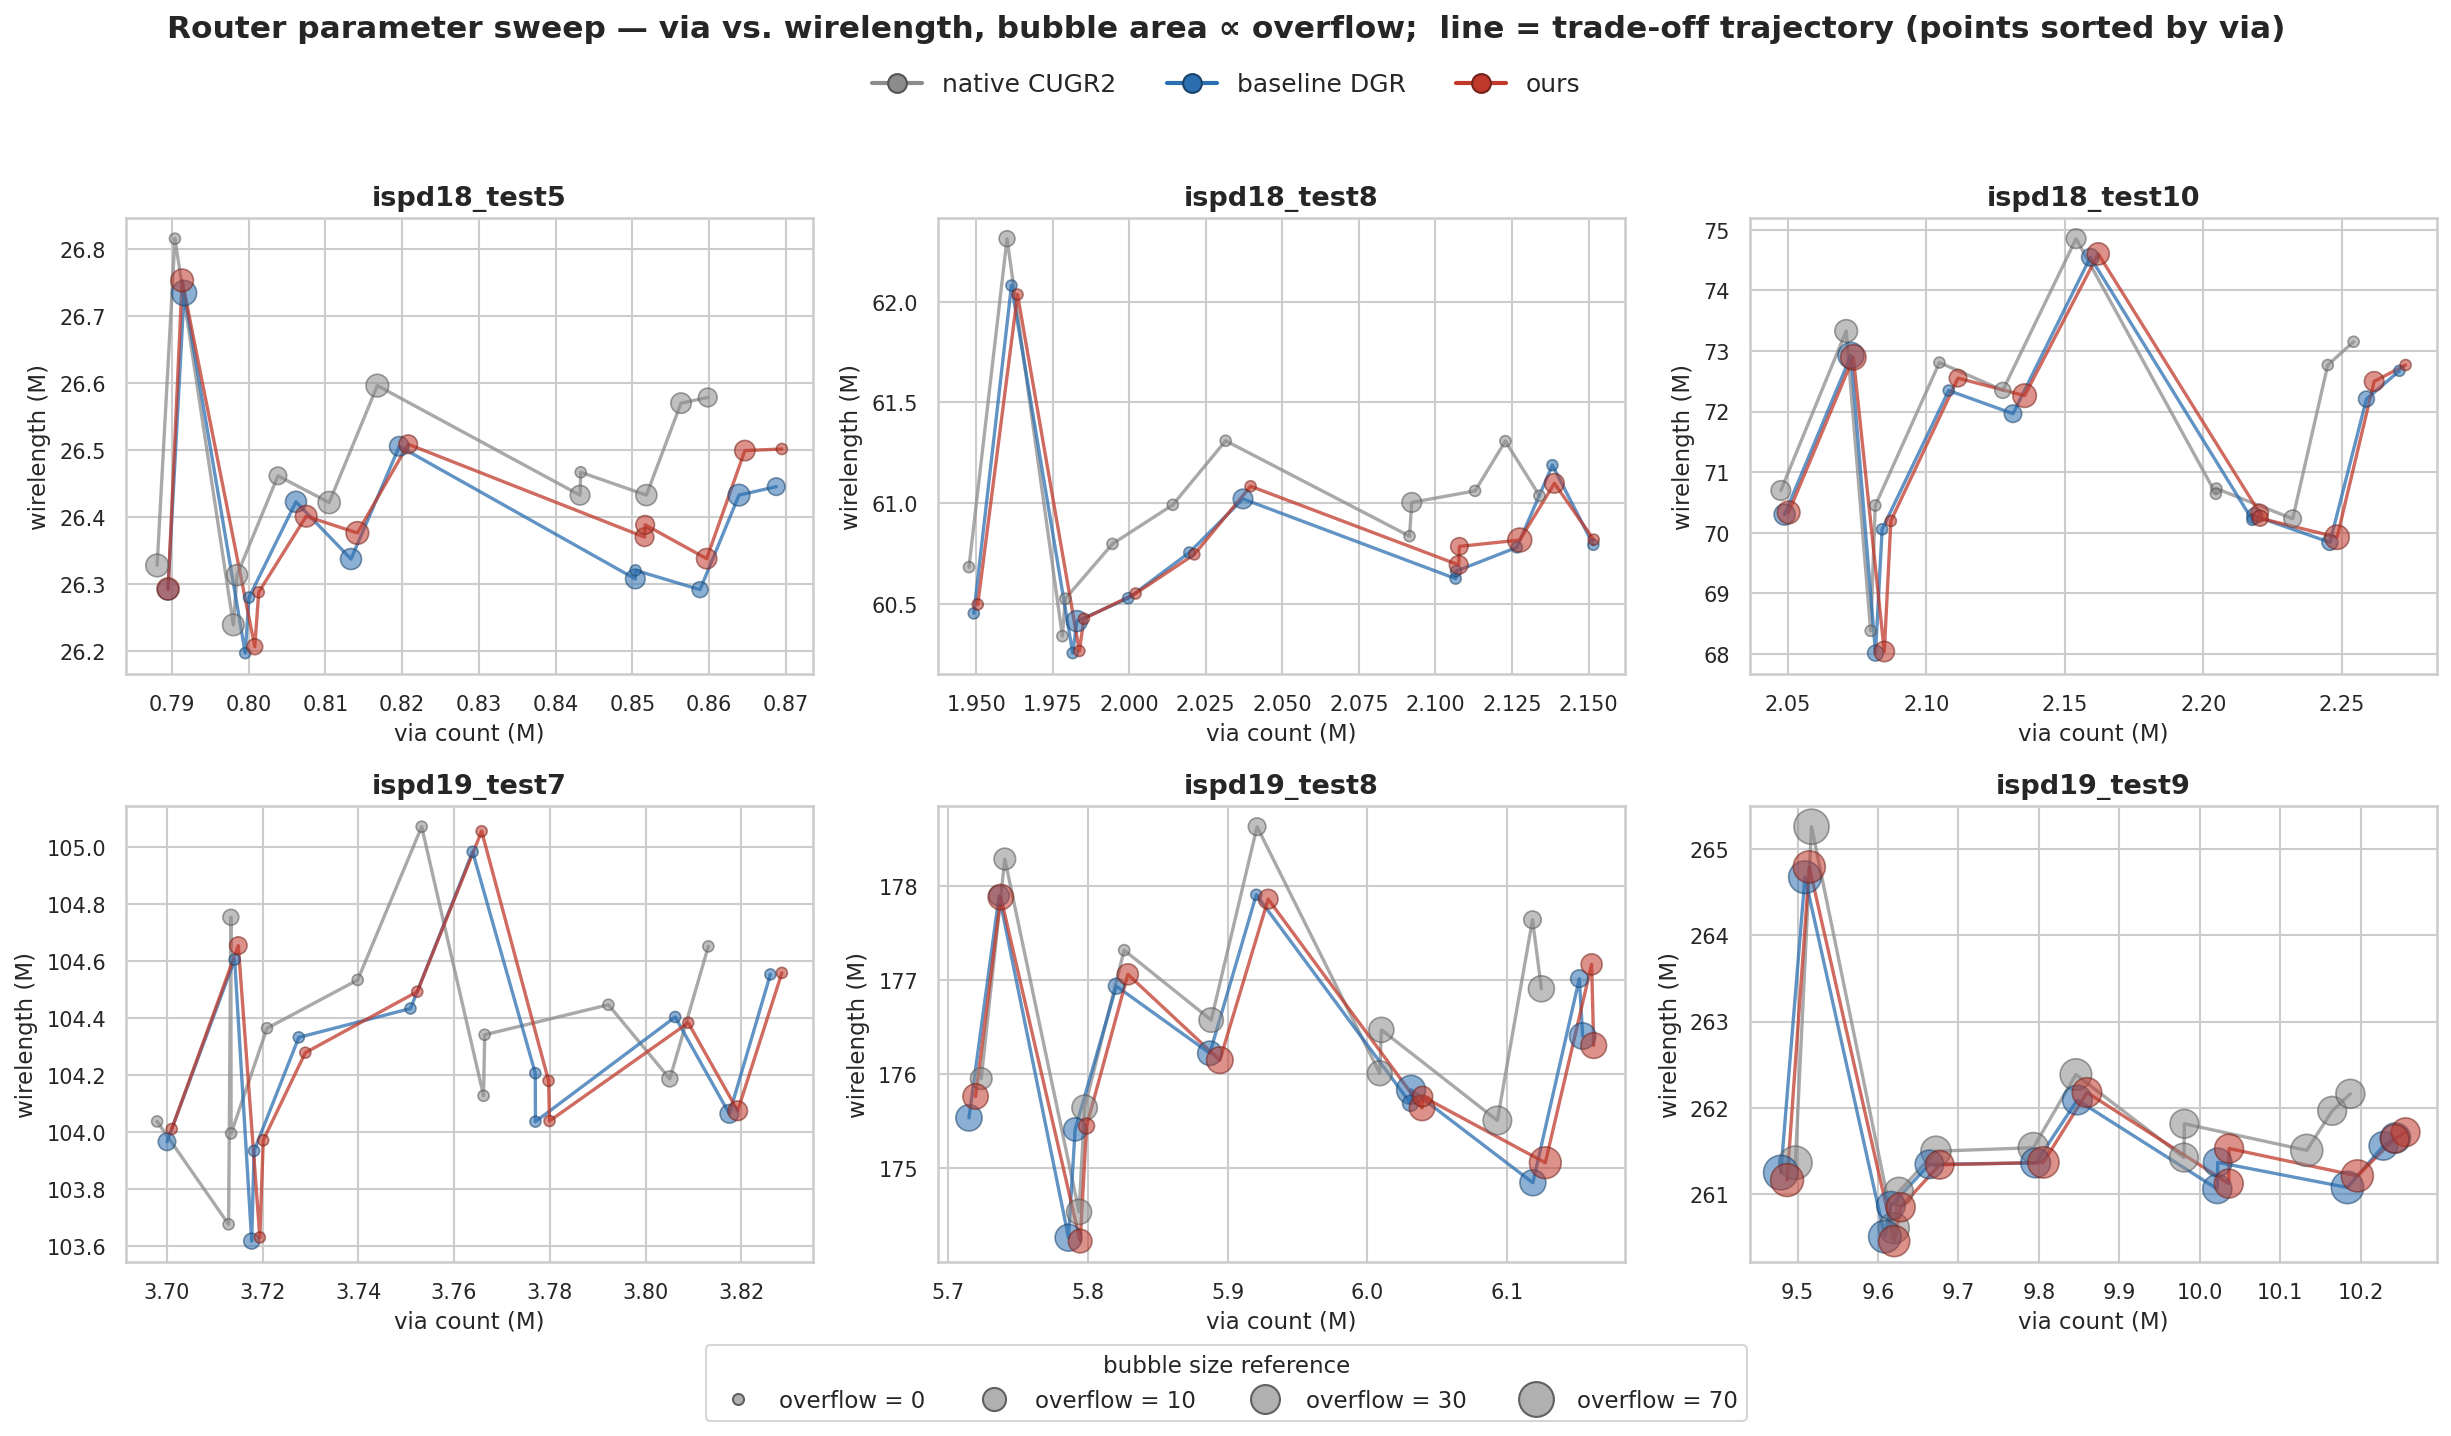
\includegraphics[width=.99\linewidth]{scatter12pro_all-1.png}
\caption{Per benchmark, all three methods under 12 identical router
parameter settings: via count vs.\ wirelength, bubble area $\propto$ overflow,
line = trade-off trajectory (points sorted by via). Lower-left with smaller
bubbles is better.}
\label{fig:scatter}
\end{figure}

Figure~\ref{fig:pareto} distills the same sweep to each method's
\emph{Pareto frontier} in (via, wirelength): the lower-left non-dominated
operating points, drawn as a staircase, with dominated points faded. This is
the cleanest side-by-side of the three methods --- a frontier lying to the
lower-left is strictly better. The frontiers of the three methods are close
(again consistent with the honest finding), with ``ours'' reaching the
lower-left corner (e.g.\ ispd18\_test10 at via $2.05$M / WL $70.3$M, and the
minimum-WL corner of ispd19\_test8) without larger overflow bubbles.
\begin{figure}[h]\centering
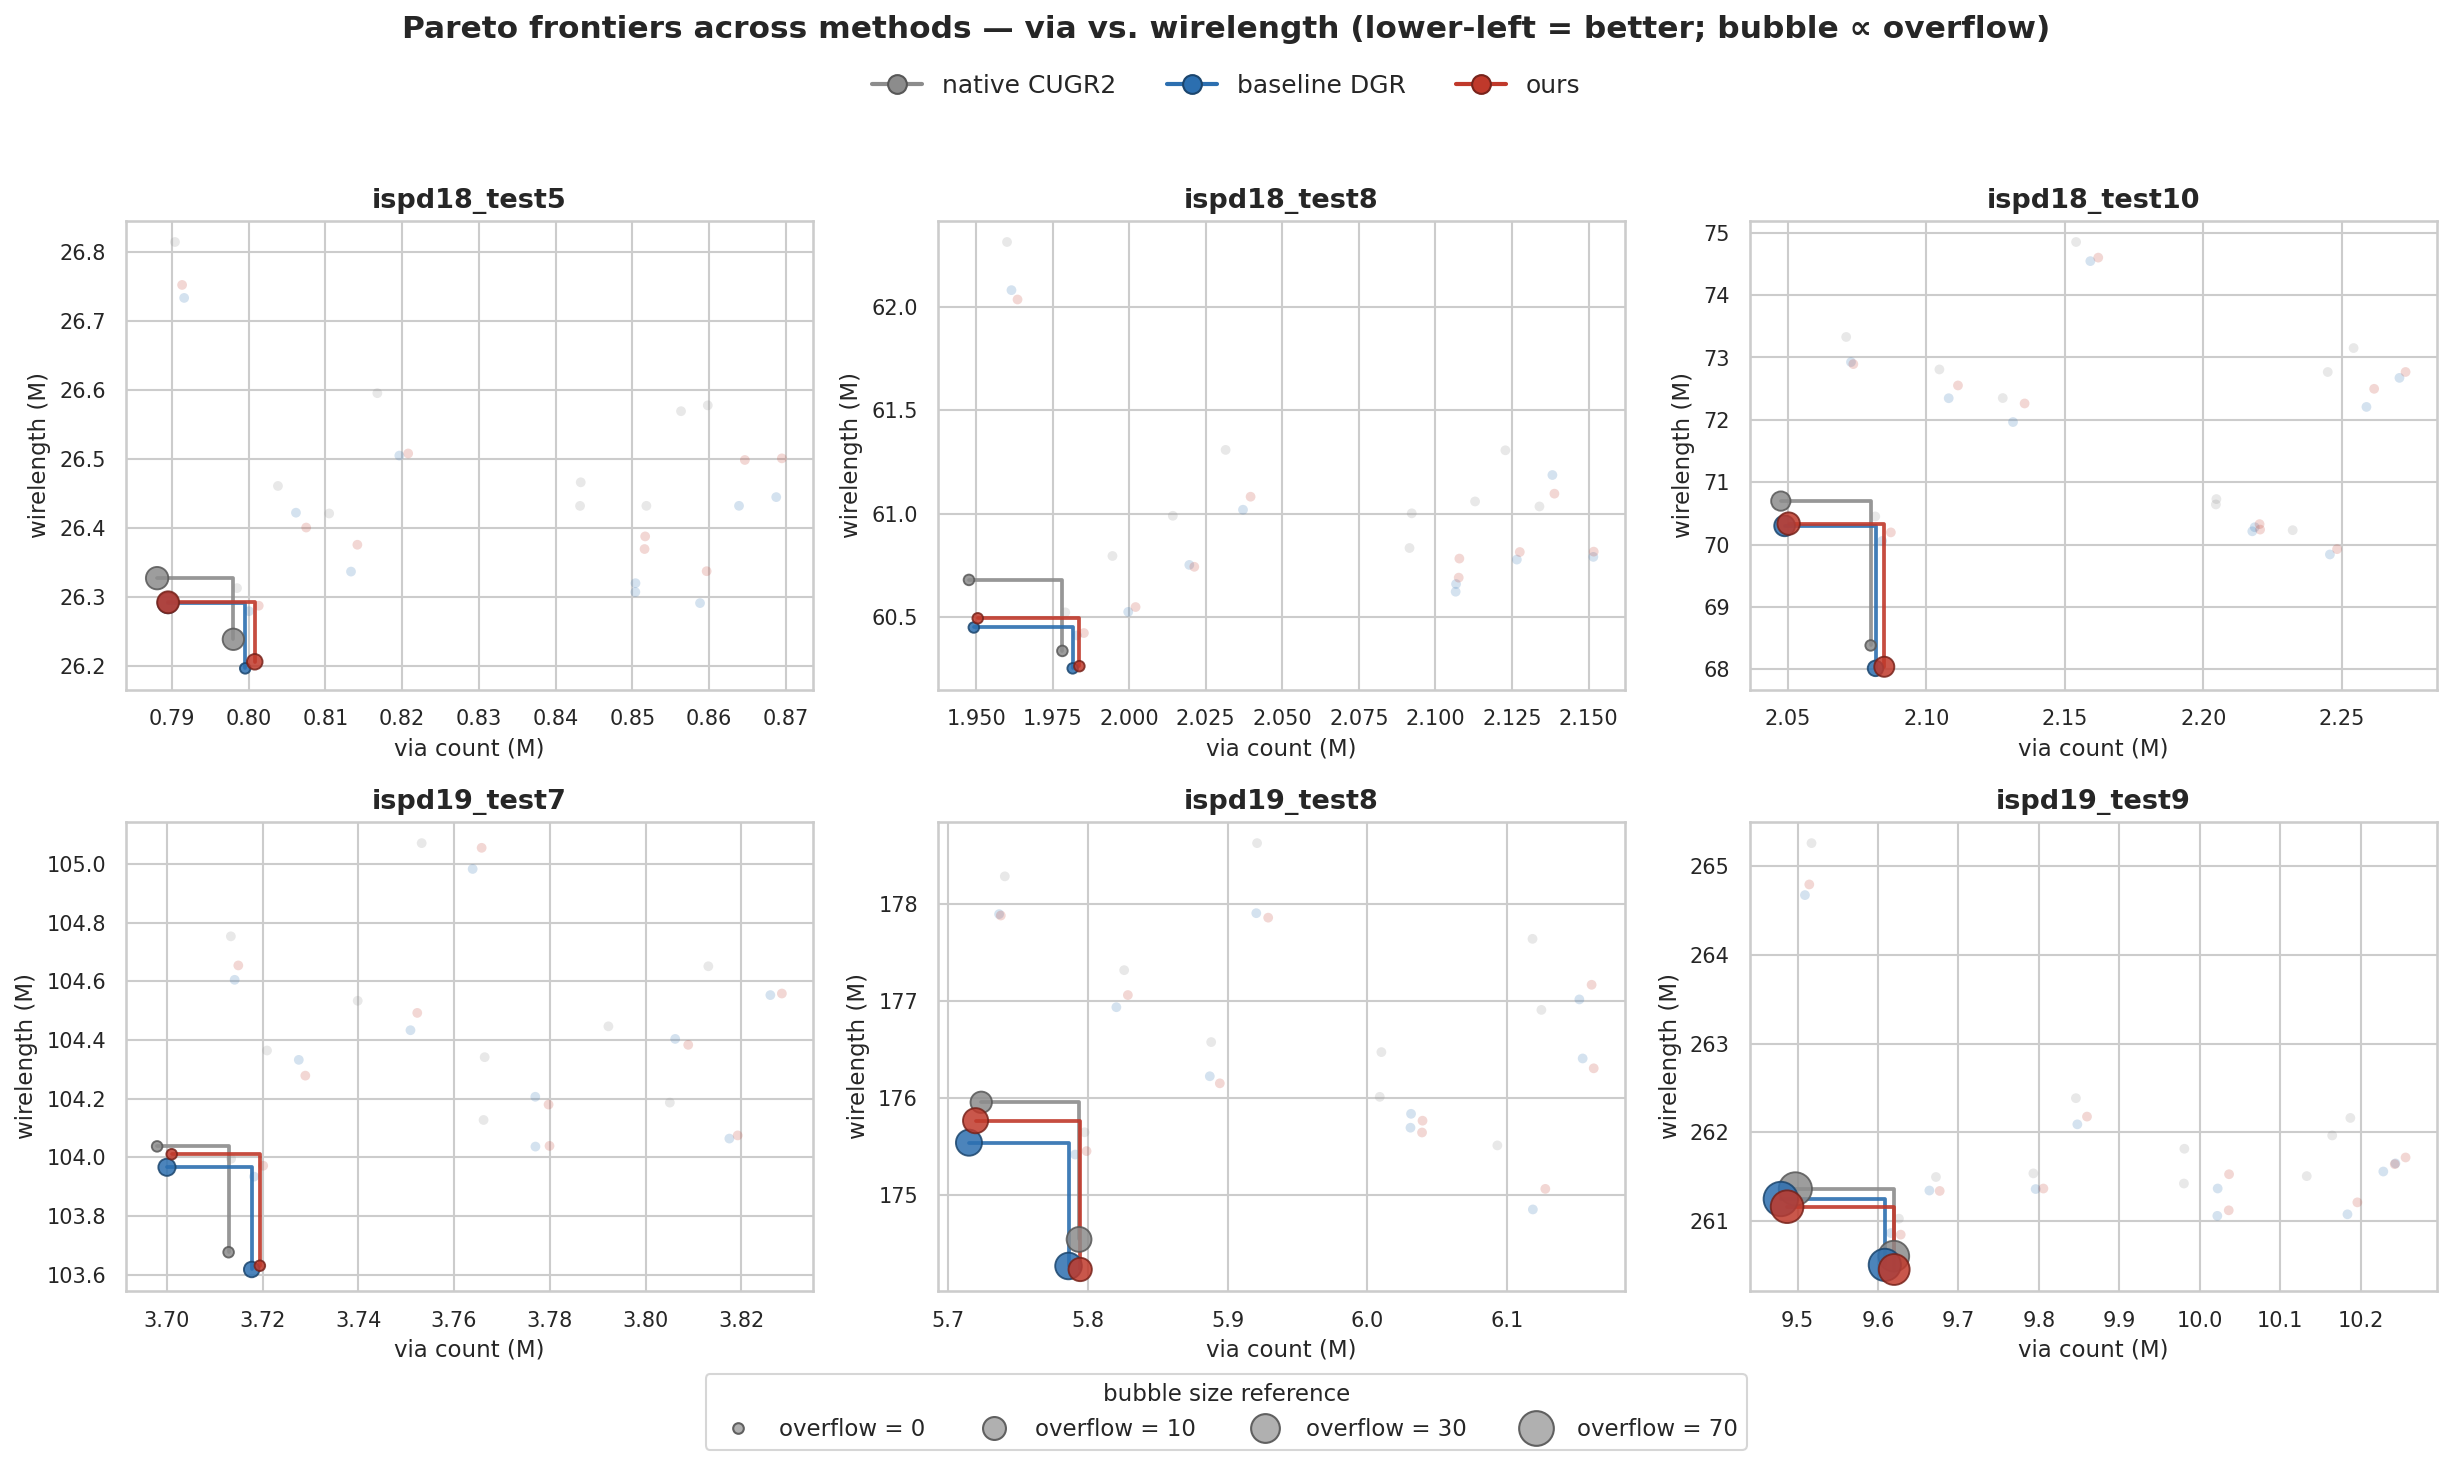
\includegraphics[width=.99\linewidth]{pareto_all-1.png}
\caption{Pareto frontiers across methods (native CUGR2 / baseline DGR / ours):
via vs.\ wirelength, non-dominated staircase per method, bubble area
$\propto$ overflow. Lower-left is better; dominated points are faded.}
\label{fig:pareto}
\end{figure}

\subsection{Runtime}\label{sec:iter}
\begin{table}[h]\centering\small
\caption{Guide-generation optimize time: cold 2000-iteration DGR vs.\
warm-started few-iteration DGR.}
\begin{tabular}{lrrr}
\toprule
chip & DGR 2000-it, cold (s) & DGR warm, few iterations (s) & CUGR2 route (s)\\
\midrule
18\_t5 & 343 & 4.8 & 9\\
18\_t8 & 485 & 5.2 & 23\\
18\_t10 & 377 & 3.5 & 30\\
19\_t7 & 834 & 5.7 & 47\\
19\_t8 & 1195 & 8.9 & 63\\
19\_t9 & 1933 & 10.9 & 100\\
\bottomrule
\end{tabular}
\end{table}
Discrete overflow-vs-iteration curves (fig.~\ref{fig:ofcurve}) show the
warm start begins ${\sim}4$--$11\%$ below cold start and is flat by
${\sim}5$--$30$ iterations: \textbf{${\sim}15$--$50$ iterations suffice}
(a $40\times$--$130\times$ cut from DGR's 2000), with the caveat that the
final few overflow edges of heavily congested designs still benefit from a
longer single run --- hence the ensemble keeps one such arm.

\begin{table}[h]\centering\small
\caption{\textbf{Entire-flow} wall time --- all overhead included (benchmark
load, candidate pool, GNN warm start, optimize, discrete refine, guide write)
plus the CUGR2 route. One-time training (${\sim}25$ GPU-min) is amortized.}
\begin{tabular}{lrrrr}
\toprule
chip & native (route only) & DGR flow & ours flow & ours vs DGR\\
\midrule
18\_t5 & 9\,s & 351\,s & 84\,s & $4.2\times$\\
18\_t8 & 24\,s & 507\,s & 130\,s & $3.9\times$\\
18\_t10 & 31\,s & 406\,s & 144\,s & $2.8\times$\\
19\_t7 & 47\,s & 880\,s & 261\,s & $3.4\times$\\
19\_t8 & 60\,s & 1258\,s & 273\,s & $4.6\times$\\
19\_t9 & 95\,s & 2031\,s & 420\,s & $4.8\times$\\
\bottomrule
\end{tabular}
\end{table}
End to end, our flow is $2.8\times$--$4.8\times$ faster than the DGR flow at
$4.4\times$--$9.2\times$ the bare native route time; the residual overhead is
dominated by discrete refinement and benchmark loading, not by optimization
itself (3--11\,s).
\begin{figure}[h]\centering
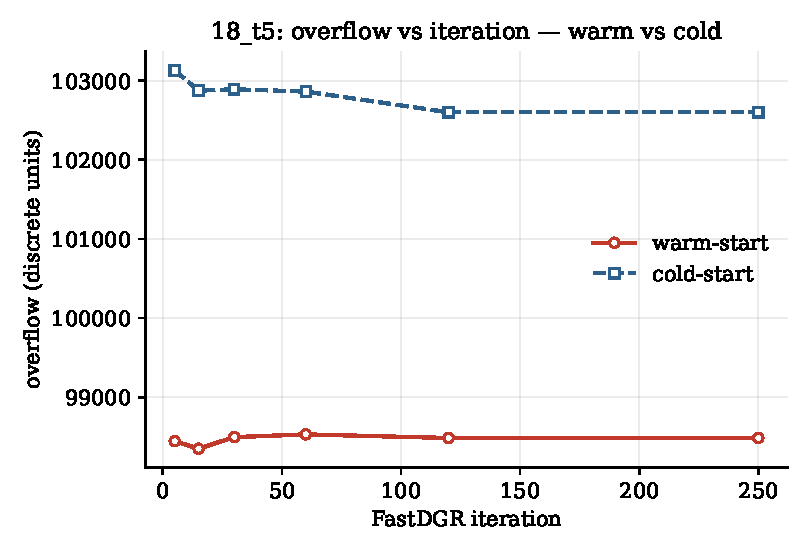
\includegraphics[width=.48\linewidth]{overflow_curve_18_t5.pdf}\hfill
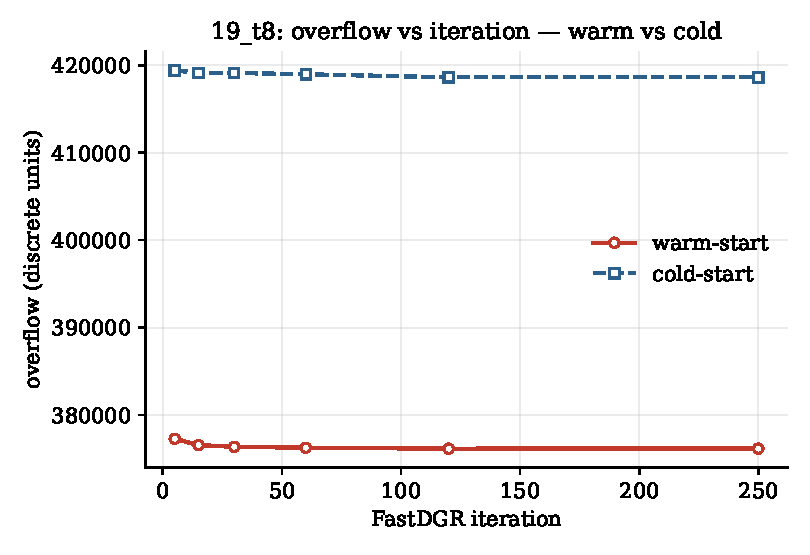
\includegraphics[width=.48\linewidth]{overflow_curve_19_t8.pdf}
\caption{Exact (discretely rounded) overflow vs.\ iteration, warm (solid)
vs.\ cold (dashed).}\label{fig:ofcurve}
\end{figure}

\subsection{Router-measured congestion heatmaps across methods}
Figure~\ref{fig:cong} compares the routed congestion of the three methods on
the most congested benchmark; the same comparison for all six benchmarks (18
maps) accompanies this report. These maps are \emph{industry-convention}
congestion views produced from the router's own per-GCell usage and capacity
(CUGR2's heatmap output): the die is dark where routing resources are free,
and cells are colored by discrete bins as they approach (yellow) or exceed
(orange/red/magenta) capacity, exactly as EDA congestion views bin
utilization. All three routes use \emph{identical} router settings; only the
guide differs. Read honestly, the maps are \textbf{nearly indistinguishable}
across methods (ispd19\_test8: 1{,}774 / 1{,}788 / 1{,}791 cells over
capacity for native / DGR / ours; no method produces severe $>$5-track
hotspots): at a fixed router operating point the guide barely moves
congestion, consistent with our fair-tuning finding. The guide's real,
measurable gains are in wirelength and vias (and runtime), which congestion
maps do not display.
\begin{figure}[h]\centering
\includegraphics[width=.98\linewidth]{congestion_compare_ispd19_test8.pdf}
\caption{Routed overflow maps on ispd19\_test8 (white = no overflow;
color = tracks over capacity), each method at its evaluated operating point;
panel labels give the official overflow. The full 18-map set (six benchmarks
$\times$ three methods) is provided alongside.}
\label{fig:cong}
\end{figure}

\subsection{Honest negatives}\label{sec:negatives}
\textbf{Data scaling is flat.} Three controlled experiments --- instances-seen
milestones, distinct-set-size on certified packs ($+0.6\%$, noise), and
distinct-set-size on congested packs with a fixed held-out and equal step
budgets ($-0.4\%$) --- all show no generalization gain beyond ${\sim}50$
distinct designs. With this feature set (4 grid + 4 candidate features) and
${\sim}10^5$ parameters, \emph{model/feature capacity, not data, is the
binding constraint}. \quad \textbf{Router knobs are not a learned
contribution.} Per-benchmark CUGR2 flag tuning (\texttt{-cls/-vm/-wsa})
improves \emph{every} method, including native CUGR2 (e.g.\ 19\_t8 overflow
$18\!\to\!0$ with no guide at all); after equal tuning all methods sit within
${\sim}0.3\%$. We therefore apply knobs symmetrically and never attribute
their gains to learning. \quad \textbf{Candidate shapes.} L-only pools
(the default) are optimal here; adding Z/C detour patterns raised vias
($+0.6\%$) and overflow. The remaining WL lever is Steiner-tree topology,
not route shapes.

\subsection{Training-efficiency results}
Graph caching (build each pack's graph once, LRU-resident) makes batch
training steps pure forward/backward: 600 steps over 3200 distinct packs run
in ${\sim}42$\,s on CPU. End-to-end (teacher-free) and supervised training
reach the same held-out quality; the all-6 full-size training run costs
${\sim}15$ GPU-minutes, and the complete quality pipeline above used a
single fractional GPU for minutes per chip.

\section{Industrial scale-out and commercialization}
The ISPD'24 contest adapter (\texttt{.cap/.net} $\to$ pipeline format,
validated against the InstantGR parser) is implemented and unit-tested;
contest benchmarks are Google-Drive hosted and pending manual download, after
which the identical flow applies. The commercial value proposition measured
here: \emph{train once (${\sim}25$ GPU-minutes), reuse everywhere} --- a
single warm-start model lets DGR run in seconds per design and deliver
better-than-SOTA routes on every design tested, with total flow time
dominated by the router itself.

\section{Conclusion}
A one-model cross-benchmark warm start made possible by grid coarsening,
teacher-free end-to-end training, few-iteration DGR, and ensemble finishing
combine to strictly dominate both native CUGR2 and DGR on all six
ISPD'18/'19 benchmarks under CUGR2's own metrics --- with fully honest
accounting of what does not help (data scaling, knob tuning, Z/C shapes).
\end{document}
